\title{Client Localization in Ad Hoc Networks as a Nonlinear Optimization Problem}
\author{
        Nikhil Buduma, Elizabeth Dethy, Anubhav Jain, David Ward
}
\date{\today}

\documentclass[12pt]{article}
\usepackage[papersize={8.5in,11in}]{geometry}
\usepackage{graphicx}
\usepackage{wrapfig}
\graphicspath{ {images/} }

\begin{document}
\maketitle

\begin{abstract}
This write-up discusses the algorithms we use to determine the configuration of clients in an ad hoc network. We develop methods that enable configuration determination with significant tolerance to errors in measurement. We first eliminate error in angle measurements by formulating a constrained nonlinear optimization problem. From these corrected angles, we determine a scale-independent configuration that we use to correct errors in distance measurements. This is computed with a second nonlinear optimzation. The final output of the algorithm is a correctly scaled configuration of clients. 
\end{abstract}

\section{Setup}
\begin{wrapfigure}{r}{0.4\textwidth} %this figure will be at the right
    \centering
    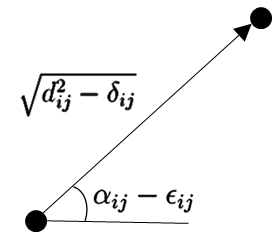
\includegraphics[width=0.25\textwidth]{figure1}

\footnotesize{\textbf{Figure 1.} Physical meaning of the quantities $\alpha_{ij}$, $\epsilon_{ij}$, $d_{ij}$, and $\delta_{ij}$.}

\end{wrapfigure}

We consider a setup in which N nodes are placed in the plane in some unknown configuration, each facing arbitrary directions. Each node $i$ can measure the angle of arrival of the signals from each of the other $N -1$ nodes with respect to the horizontal. We let the measurement by node $i$ of its angle with respect to node $j$ be $ 0 \le \alpha_{ij} \le 2\pi$. We let the error for this measurement be $\epsilon_{ij}$, where $\alpha_{ij} - \epsilon_{ij}$ is the true angle from node $i$ to $j$.

Similarly, each of the nodes also has an estimate, with some error, of its distance to the other nodes. We denote the distance from node $i$ to $j$ as estimated by node $i$ to be $d_{ij}$. The error of the square of the measurement is denoted as $\delta_{ij}$, meaning that the true distance between $i$ and $j$ can be expressed as $\sqrt{d_{ij}^2 - \delta_{ij}} = \sqrt{d_{ji}^2 - \delta_{ji}}$.

For all $i$ and $j$, the measurements $\alpha_{ij}$ and  $d_{ij}$ are known, but the values of $\epsilon_{ij}$ and $ \delta_{ji}$ must be computed. 

\section{Angle Error Elimination}
We first set out to compute $\epsilon_{ij}$ for all $i$ and $j$. We proceed by formulating the computation of all $\epsilon_{ij}$ as a nonlinear optimization problem. We generate a total of $n \choose 3$ linear constraints by considering every triangle with nodes $i$, $j$, and $k$. Without loss of generality, we consider the angle at vertex $i$ and assume that $\alpha_{ij} > \alpha_{ij}$. This angle evaluates to $\alpha_{ij} - \alpha_{ik} +  \epsilon_{ik} - \epsilon_{ij}$ or $2\pi - (\alpha_{ij} - \alpha_{ik} +  \epsilon_{ik} - \epsilon_{ij})$, depending on whichever of $\alpha_{ij} - \alpha_{ik}$ or $2\pi - (\alpha_{ij} - \alpha_{ik})$, respectively, comes out to be less than $\pi$. The sum of the 3 computed angles must sum to $\pi$, leading to a linear equality constraint involving 6 variables (which are $\epsilon$-errors). In addition, for the purpose of simplicity, we presume that the $\alpha_{ij} - \epsilon_{ij} \ge 0$ and $\alpha_{ij} - \epsilon_{ij} \le 2\pi$ for all $i,j$. This generates an additional $4{n \choose 2}$ constraints. 

Now we define the objective function that we aim to minimize given these constraints. We would like the corrected angles to remain close to the original measurments, but at the same time, we would also like to force the errors to affect as few measurements as possible (errors are most likely to be severe at specific nodes due to interference and multipath). Thus we define the objective function with a tunable parameter $\lambda_\alpha$ to minimize the linear combination of the square of the error vector's L2 norm as well as the entropy (a sparsity-forcing function):

$$\sum_{i,j}{\epsilon_{ij}^2} + \lambda_\alpha\sum_{i,j}{\log(1+ \epsilon_{ij}^2)} $$

We can now use the $\epsilon$-values computed by the nonlinear optimization in order to find the corrected angles between nodes.

\section{Computing the Scale-Independent Configuration}
Given the corrected angle measurements, we would like to generate a scale-independent configuration in terms of Cartesian coordinates for node $i$, where $i$ is placed at the origin. To do so, we arbitrarily select another node $j$ and we place $j$ at the coordinates $(\cos(\alpha_{ij}), \sin(\alpha_{ij}))$. From this, we can immediately compute the position of every other node $k$. Specifically, we know that $k$ lies along the vector $\langle \cos(\alpha_{ik}), \sin(\alpha_{ik}) \rangle$. We then aim to compute $s_k$, the necessary multiplier for this vector to determine the exact position of $k$ in the scale-independent configuration. We can compute $\theta_{k,1}$ which is the angle at node $i$ and $\theta_{k,2}$ which is the angle at node $j$ using the method described in the previous section. Then using the law of sines:

$$s_k = \frac{\sin(\theta_{k,2})} {\sin(\pi-\theta_{k,1}-\theta_{k,2})}$$

This places node $k$ at the coordinate $(x_k^*, y_k^*) = (s_k\cos(\alpha_{ik}), s_k\sin(\alpha_{ik}))$. We repeat the procedure for every node $k$, and we can then plot every node in the Cartesian plane. However, we note that this computed configuration does not reflect the true distances between nodes, just their relative positioning. Determining absolute distances from measurements is the subject of the following section.

\section{Distance Error Elimination}
Finally, by employing the configuration from above, we compute the $\delta$-errors that determine the properly scaled configuration. To do so we formulate another nonlinear optimization problem with the variables $\delta_{ij}$ for all $i,j$ and the variable $C$, the scaling with respect to the scale-independent configuration above. We can express true positions in terms of the scale-independent positions: $(x_i, y_i) = (Cx_i^*, Cy_i^*)$. For every ordered pair $(i,j)$, we can generate the following linear constraint:

$$\delta_{ij} + ((x_i^* - x_j^*)^2+ (y_i^* - y_j^*)^2) \cdot C = d_{ij}^2$$

Moreover, we require $C > 0$. This gives us a total of $4{n \choose 2} + 1$ linear constraints. We can then minimize the objective function:

$$\sum_{i,j}{\epsilon_{ij}^2} + \lambda_d\sum_{i,j}{\log(1+ \epsilon_{ij}^2)} $$

With the computed value of $C$, we now have the properly scaled configuration that we originally set out to find. 

\section{Simple Example}

In order to demonstrate the ability of the algorithm to reconstruct the configuration of clients despite significant errors in measurement, we construct toy examples that include 3, 4, or 5 nodes placed in the coordinate plane. We first compute what the measurements would be in an ideal world where there is zero error. We then selectively introduce errors in various measurements, treate this as our input, and compare the output configuration of the algorithm with the original ground truth. Every example produced ouptut that was highly comparable with the original configuration. 

\begin{wrapfigure}{r}{0.4\textwidth} %this figure will be at the right
    \centering
    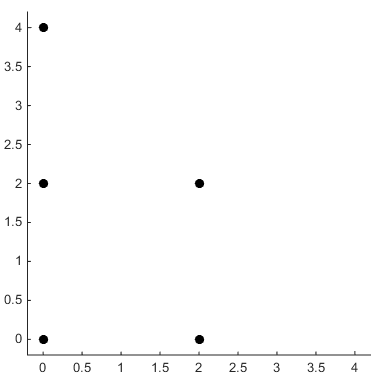
\includegraphics[width=0.25\textwidth]{figure2}

\footnotesize{\textbf{Figure 2.} Ground truth configuration.}

\end{wrapfigure}

We walk through a specific example here for the purpose of illustration. Consider a ground truth configuration of 5 nodes distributed in the Cartesian coordinate plane as shown in Figure 2. The positions of the nodes with respect to an arbitrarily chosen origin are as follows: $(x_0, y_0) = (0,0)$, $(x_1, y_1) = (2,0)$, $(x_2, y_2) = (2,2)$, $(x_3, y_3) = (0,2)$, and $(x_4, y_4) = (0,4)$. Our goal is to compute the configuration observed by node 0, where node 0 is placed at the origin of the new reference frame. If each node computed its angles in degrees with respect to all of the other nodes without any error, we would find the following matrix where the diagonal entries are invalidated (since it is illogical for a node to compute an angle with respect to itself):

\[ A_{optimal}= \left( \begin{array}{ccccc}
- & 15 & 60 & 105 & 105 \\
90 & - & 0 & 45 & 26.57 \\
135 & 180 & - & 90 & 45 \\
0 & 45 & 90 & - & 180 \\
0 & 26.57 & 45 & 0 & - \end{array} \right)\] 

Moreover, the error-free distance matrix would be as follows:

 \[ D_{optimal}  =\left( \begin{array}{ccccc}
0 & 2 & 2\sqrt{2} & 2 & 4 \\
2 & 0 & 2 & 2\sqrt{2} & 2\sqrt{5} \\
2\sqrt{2} & 2 & 0 & 2 & 2\sqrt{2} \\
2 & 2\sqrt{2} & 2 & 0 & 2 \\
4 & 2\sqrt{5} & 2\sqrt{2} & 2 & 0 \end{array} \right)\] 

Now in application, the measurements by these nodes would not be perfect and we would introduce a significant amount of error in certain measurements. This could result in the following measurements, for instance:

\[ A_{real}= \left( \begin{array}{ccccc}
- & 15 & 65 & 105 & 100 \\
90 & - & 0 & 40 & 20 \\
135 & 180 & - & 86 & 45 \\
0 & 40 & 90 & - & 180 \\
0 & 20 & 45 & 356 & - \end{array} \right)\] 

 \[ D_{real}  =\left( \begin{array}{ccccc}
0 & 2 & 2.6 & 2 & 6 \\
2 & 0 & 2 & 2.8 & 4.5 \\
2.8 & 2 & 0 & 2 & 2.8 \\
2 & 3 & 2 & 0 & 1.7 \\
4 & 5 & 2.8 & 2 & 0 \end{array} \right)\] 

\paragraph{}
After running the routine, we (quite surprisingly) generate the output that is shown in Figure 3. The algorithm faithfully reconstructs the expected configuration, with minimal error, proper orientation, and the correct scaling. 

\begin{figure}[h]
\centering
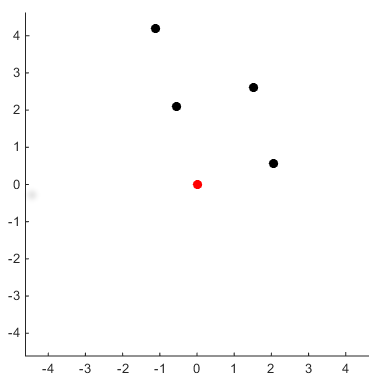
\includegraphics[width=10cm]{figure3}

\footnotesize{\textbf{Figure 3.} Output generated by our algorithm.}
\end{figure}

\section{Next Steps}
There are a couple of issues that must be investigated to move towards a full implementation. First, and most significantly, the interface described by our algorithm requires slightly more information than we currently can immediately generate from our experimental setup. Because we are not using directional antennas, we do not obtain rays (directed vectors) that determine the location of nodes. Instead, we generate entire lines, which makes it difficult to determine the exact orientation of the computed configuration. To solve this issue, we may need to define a "command node" and make certain assumptions about th e position of this node. 

In addition, we will need to refine our algorithms as we begin to collect data from our experimental setups. Specifically, our objective functions make certain assumptions about the nature of the measurement errors that, in reality, may not be accurate. Thus, we may need to modify our objective functions and tune parameters based on additional observations.

\end{document}
